The results of the implemented Barnes-Hut algorithm can be seen in Figures~\ref{fig:weak_scaling} and \ref{fig:strong_scaling}.

In Figure~\ref{fig:weak_scaling}, the large jump and irregularities in the plot are most likely due to the inefficient communication that was implemented. In the current implementation, at the start of each iteration an {\tt MPI\_Allgather} was performed so that each node/process had all the paricles so they could see which it needed for what octants. After implementing the code, it was realized that there could be an {\em interprocessor sorting} done between the nodes, removing the {\tt MPI\_Allgather} requirement. There were a few other {\tt MPI\_Allgather} and {\tt MPI\_Allreduce} commands that were performed which were realized after that they could be removed.

With more time, these could be fixed so that the code was more efficient. The code and timings were performed on {\sc Mir} since {\sc Tangent} did not have {\sc Petsc} installed and was unable to be installed locally.

The strong scaling results in Figure~\ref{fig:strong_scaling} seem to agree with how the scalability should look. The timings follow the general pattern for the time taken to solve the problem.

In order to compare the results, the sequential case for the $\mathcal{O}\left( N^{2}\right)$ algorithm was implemented and timed as well. Those timings can be seen in Table~\ref{table:sequential}. The implemented code performed {\em worse} than the $\mathcal{O}\left( N^{2}\right)$ algorithm for $p < 12$ and $N < 8000$. This is likely due to the extra requirement to build the tree with every iteration and savings not coming about except for large $N$.

%    Results: Describe the experiments you performed to evaluate your code/methods. Summarize results and discuss them. Are the results what you expected. If not, why are they better or worse then what you expected. What other experiments would you have done if you had more time. With the knowledge of the results, would you change your methods in any way to improve performance or scalability. 


\begin{figure}[H]
\centering
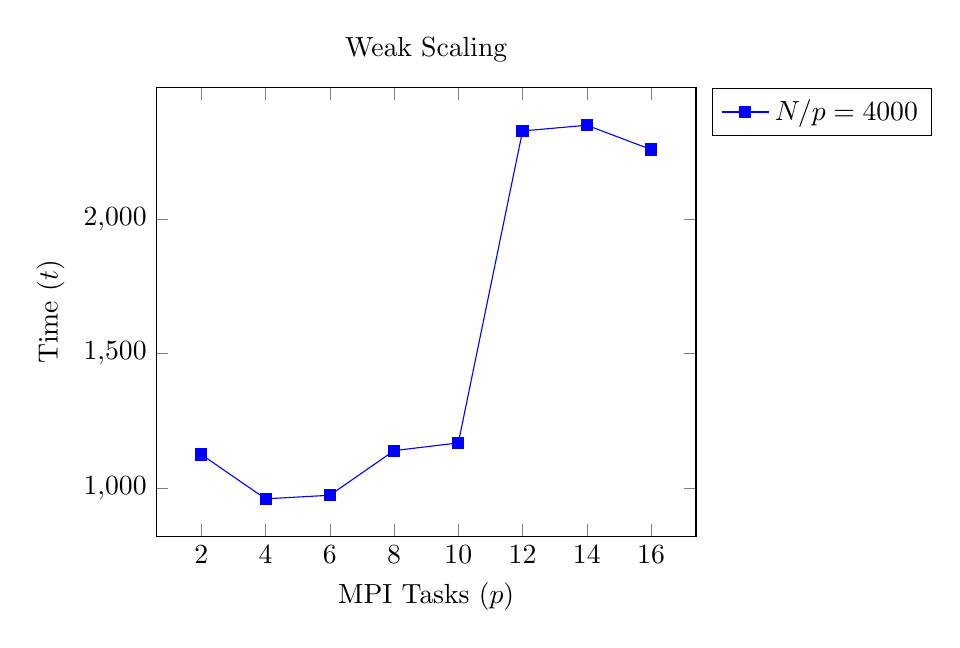
\begin{tikzpicture}
\begin{axis}[title={Weak Scaling}, xlabel={MPI Tasks $(p)$}, ylabel={Time $(t)$}, legend pos=outer north east]
\addplot[color=blue, mark=square*,]coordinates{(2, 1124.41)(4, 959.32)(6,972.64)(8,1138.98)(10,1167.73)(12,2330.16)(14,2351.48)(16,2260.98)};
\legend{$N/p=4000$}
\end{axis}
\end{tikzpicture}
\caption{$N/p$ remains constant}
\label{fig:weak_scaling}
\end{figure}

\begin{figure}[H]
\centering
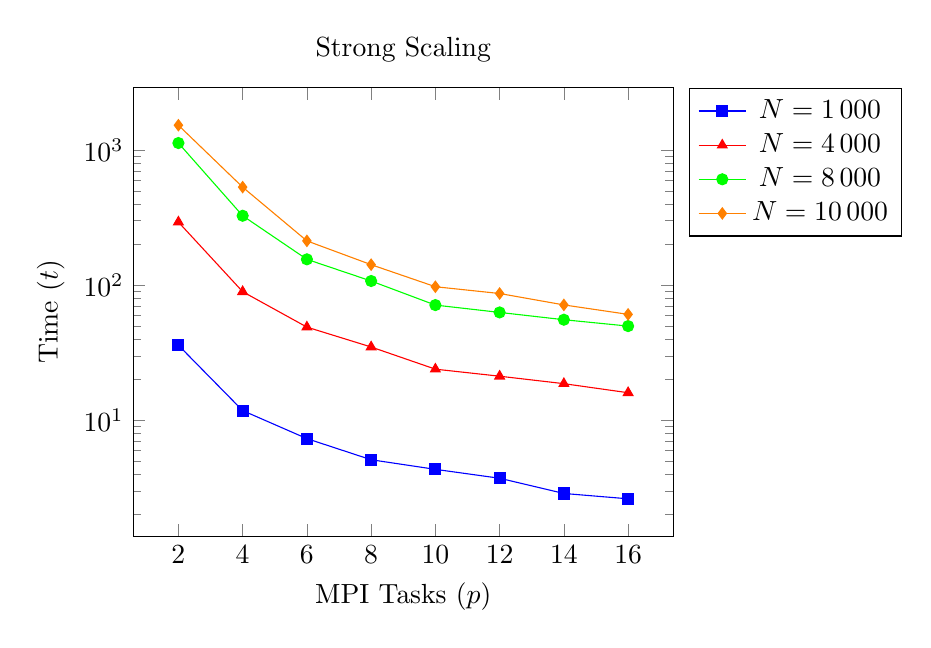
\begin{tikzpicture}
\begin{axis}[title={Strong Scaling}, xlabel={MPI Tasks $(p)$}, ylabel={Time $(t)$}, ymode=log, legend pos=outer north east]
\addplot[color=blue, mark=square*]coordinates{(2,35.93)(4,11.79)(6,7.31)(8,5.10)(10,4.33)(12,3.72)(14,2.87)(16,2.62)};
\addplot[color=red, mark=triangle*]coordinates{(2,293.31)(4,89.53)(6,48.94)(8,34.87)(10,23.89)(12,21.19)(14,18.66)(16,15.99)};
\addplot[color=green, mark=*]coordinates{(2,1128.71)(4,326.75)(6,155.42)(8,107.37)(10,71.25)(12,62.87)(14,55.51)(16,49.80)};
\addplot[color=orange, mark=diamond*]coordinates{(2,1529.18)(4,532.14)(6,212.84)(8,141.9024)(10,97.43)(12,86.79)(14,71.45)(16,60.82)};
\legend{$N = 1\,000$, $N = 4\,000$, $N = 8\,000$, $N = 10\,000$}
\end{axis}
\end{tikzpicture}
\caption{$N$ remains constant}
\label{fig:strong_scaling}
\end{figure}

\begin{table}[H]
\centering
\caption{Timings for Sequential}
\begin{tabular}{@{}l | r@{}}
\hline\hline
$N$ & $t$\\
\hline
1000 & 1.04\\
4000 & 16.61\\
8000 & 66.07\\
10000 & 103.11\\
\hline
\end{tabular}
\label{table:sequential}
\end{table}


%\subsubsection*{Future Work}